\documentclass{article}

\usepackage{amsmath,amssymb,amsthm,graphicx}
\usepackage{fullpage}
\usepackage{caption,subcaption}
\newtheorem{prob}{Problem}
\newtheorem{theorem}{Theorem}[section]
\newtheorem{lemma}{Lemma}[section]

\newenvironment{problem}
{
\renewcommand{\labelenumi}{(\alph{enumi})}
\renewcommand{\labelenumii}{\roman{enumii}.}
\begin{prob}
}
{
\end{prob}
 }
 \newcommand{\N}{\mathbb{N}}
 \newcommand{\Z}{\mathbb{Z}}
 \newcommand{\Q}{\mathbb{Q}}
 \newcommand{\R}{\mathbb{R}}
 \newcommand{\C}{\mathbb{C}}
 \newcommand{\bM}{\begin{bmatrix}}
 \newcommand{\eM}{\end{bmatrix}}
 \newcommand{\Ni}{\N\cup\{\infty\}}
  \newcommand{\rmD}[1]{\mathrm{d}#1}
\newcommand{\floor}[1]{\lfloor #1 \rfloor}
\title{Optimal Path Planning for Robotic Arms in Household Assistance}
\author{Vikram Sunder and Zachary Greenberg}

\begin{document}

\maketitle

\section{Abstract}
We investigated and implemented motion planning algorithms for a robotic arm. The algorithm computes a shortest path in a given metric space.  To find the optimal path, we considered various metrics on a graph in Configuration Space. For example we considered the Euclidean distance in work space, energy needed to transition between states, and the energy required to hold an object in the gripper. Currently we have a small mobile robot with a five degrees of freedom arm. The overall objective is for the robot to help with small household tasks. We simulated the motion of the arm in Matlab to evaluate the various paths. 

\section{Introduction}
One of the main problems with bringing robots into the home is the cost of hight precision parts. Currently the cost of quality robotic arms is far beyond the price range of the average household. While they might be more accessible in the future, we want to experiment with a lower cost robotic arm currently available. The trade off here is decreased power and precession. Our robot has a small 5 degree of freedom arm, that we hope to use to pick up plates/cups or open doors. However, to maximize the set of objects we can manipulate and the duration of time that we can carry out interactions we need minimize the length of individual interactions and the energy required to carry them out.  The longer our arm takes to manipulate an object the more power it will consume from its highly limited power source.  Likewise the more torque required from the servos will translate to increased current draw and minimize the weight of the objects we can manipulate.  As such we must optimize our trajectories to meet these goals.  

\section{The Robot}
Our robot uses Willow Garage's Turtlebot as a base. On top of this we have attached a PhantomX Reactor robotic arm. This arm has 5 degrees of freedom. It can rotate about the base to select a particular plane of motion.  There are then three degrees of freedom in this particular plane.  The last degree of freedom is a wrist joint. \ref{fig:DHparam} for the Denavit-Hartenberg parameters for the robot. \\
\begin{figure}[hb]
\centering
\begin{tabular}{|r|c|c|c|c|}
\hline
&$\alpha$ & a & d & $\theta$\\
\hline
\hline
1& $\frac{\pi}{2}$ & 0 & 26.5 & $\theta_0$\\
\hline
2& 0 & 150 & 0 & $\frac{\pi}{2}+\theta_1$\\
\hline
3& 0 & 150 & 0 & $\theta_2$\\
\hline
4& $\frac{\pi}{2}$& 0 & 0 & $\frac{\pi}{2}+\theta_3$\\
\hline
5& 0& 0& 116.525 & $\theta_4$\\
\hline
\end{tabular}
\caption{Denavit Hartenberg Paramaters}
\label{fig:DHparam}
\end{figure} \\
For path planning there are a few convenient things about the forward kinematics for this robot. The first is that the final angle, $\theta_4$ doesn't affect the final position of the robot. Therefore when searching configuration space, any algorithm doesn't need to search changes in $\theta_4$. Similarly $\theta_0$ only affects what plane the robot needs to be in. In a configuration space only constrained by angle limits, it is a simple computation to figure out what plane the goal point is in. Then $\theta_0$ can be calculated to point the arm in that plane. Thus we only have to search the space defined by $\theta_1,\theta_2,\theta_3$. This cuts the search space from a five dimensional space to a three dimensional space. It also solves one workspace variable, which leaves only $x,z,\alpha$ where $\alpha$ is the pitch of the end effector. 
\section{Path Planning}
Instead of computing the inverse kinematics for the arm, we decided to search the configuration space using a shortest path algorithm and use the forward kinematics to stop. From above we saw that only 3 angles had to be searched over. From there we discretized the space by placing nodes at even intervals along all three dimensions. Let a tick be the length of the intervals in radians. Then we connected any two nodes that differed by one tick in some coordinate. This created a graph to search over. Currently we are using a tick size of $\frac{\pi}{100}$ radians, but eventually a tick will correspond to the precision of the servos. This tick size gave us enough precision to find smooth paths, without making the graph too big.\\
We considered several search algorithms for the graph and eventually settled on $A^*$. We looked into $D*$, but since we chose not to consider any moving obstacles, we did not have to recompute the paths as we searched. This meant that the added complexity of $D*$ wasn't helpful. $D*$ also isn't any faster then $A*$ to find the initial path. The other search algorithm we considered was RRT. RRT is fast, but does guarantee an optimal path. The advantage of RRT is its ability to search high-dimensional non-convex spaces.  Given the number of degrees of freedom available to us this is not advantageous or necessary. Once we optimized our $A^*$ code for speed, it was fast enough to search the entire space. This combined with the simplicity of $A^*$ made it the best choice.\\
The next thing that we needed to do was find a consistent and admissible heuristic. The simplest metric we could use was the Euclidean distance in the work space between the nodes. The standard heuristic for this space is the euclidean distance to the target. When we changed the metric, we wanted an easy way to determine a heuristic. So for every new metric we added the cost to the euclidean distance. Let $c(v,w)$ be the added cost function. Let $d(v,w)$ be the euclidean distance between the nodes. So the weight of an edge $(u,v)$ is $c(v,w)+d(v,w)$. Then let $h(v)$ be the distance from $v$ to the target, $g$. So for an edge $(u,v)$ we have:
\begin{align*}
h(v) =& d(v,g)\\
\leq& d(v,w) + d(w,g) & \text{[triangle inequality]}\\
\leq& d(v,w) + c(v,w) + d(w,g) & [c(v,w)>0]\\
\leq& w(\{u,v\}) +h(g)
\end{align*}
So as long as our additional cost is always positive, the standard distance heuristic is always consistent. 

\section{Metrics }
\subsection{Euclidean Work Space}
The first metric we tried was looking at the euclidean distance in the work space. So if $FK$ was the function that maps angles to work space, the cost between nodes $u$ and $v$ is $d_{e}(FK(u),FK(v))$. In path planning in addition to specifying a position we might want to specify an orientation of the arm. For this arm the orientation we care about is the sum of $\theta_1,\theta_2,\theta_3$, which we will call $\alpha$.
So we will add to the distance between nodes $|\Delta\alpha|$ and add $|\alpha- \alpha_{target}|$ to the heuristic. Everything is still consistent so $A^*$ still works. This gives two different metrics, the basic distance, which considers orientation, and the no-alpha metric, which does not. See Figure {fig:basicPaths} to see the difference in the paths found for each metric.\\
\begin{figure}[htb]
\centering
\begin{subfigure}[b]{0.5\textwidth}
\centering
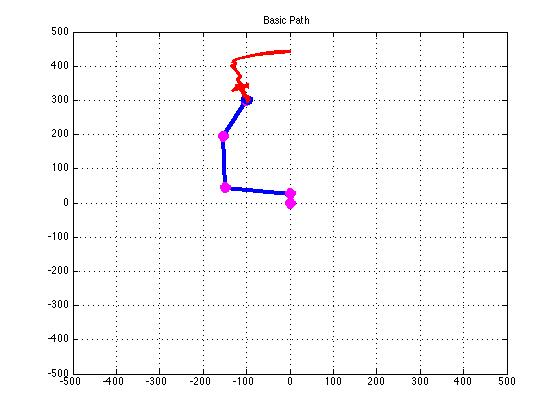
\includegraphics[scale=.5]{PathPics/Basic_Path.jpg}
\caption{Orientation Path}
\end{subfigure}%
~ 
\begin{subfigure}[b]{0.5\textwidth}
\centering
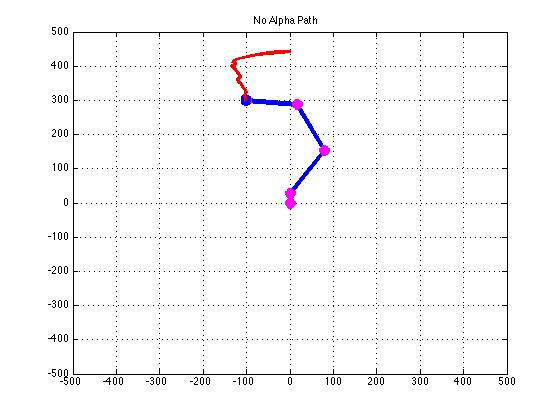
\includegraphics[scale=.5]{PathPics/NoAlpha_Path.jpg}
\caption{No Orientation Path}
\end{subfigure}

\caption{Euclidean Distance Paths}
\label{fig:basicPaths}
\end{figure}\\ 

\subsection{State Maintenance Method 1}

	From here, so long as we add positive weights to the existing costs of edges in our graph our heuristic will remain consistent and admissible.  Power is a major constraint for our robot. The amount of force the arm can output is highly limited, as is the amount of power available to the robot to carry out its various actions and functions.  As such we want to make all our motions as energy efficient as possible.  To do this we used the fact that the torque output of every actuator correlates to its energy consumption.  Therefore we will attempt to minimize the sum of the total torque of each state on a given path.  Let J be the Jacobian of the forward kinematic map of our robotic arm.  The Jacobian transpose will provide us with a linear map from forces applied by the arm to the output torques of the individual joints.  Thus we can calculate the torques required to generate a force at the end effector to counteract the force of gravity on object we are manipulating.   The cost of the edge between two configuration states $u$ and $v$ is as follows:
	
\[	d(u,v) =  \left\|(FK(u)-FK(v))\right\|^2 + \left\|J^T_v\bM 0 \\ 0 \\ mg \eM\right\|^2\]
Figure \ref{fig:EnergyPaths1} shows the different paths obtained by considering this energy. 
\begin{figure}[htb]
\centering
\begin{subfigure}[b]{0.5\textwidth}
\centering
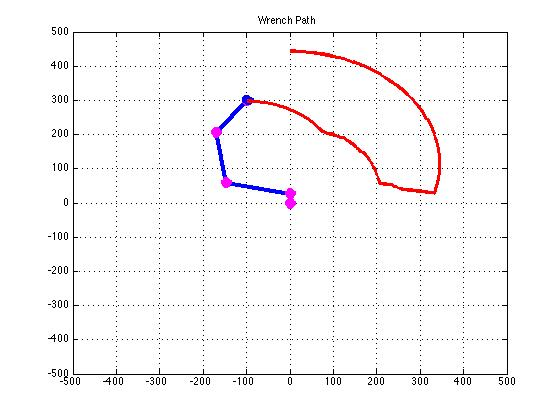
\includegraphics[scale=.3]{PathPics/Wrench_Path.jpg}
\caption{Orientation Path}
\end{subfigure}%
~ 
\begin{subfigure}[b]{0.5\textwidth}
\centering
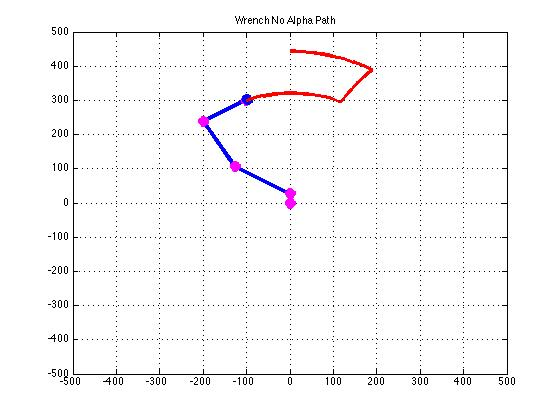
\includegraphics[scale=.3]{PathPics/Wrench_NoAlpha_Path.jpg}
\caption{No Orientation Path}
\end{subfigure}

\caption{Paths When Considering Energy To Hold Up an Object}
\label{fig:EnergyPaths1}
\end{figure}\\
\subsection{State Maintenance Method 2}

	One of the issues with this is that it does not take into account the transition from one state to the next.  To do this we use the ratio of the torque at the new state to the torque at the old state.  This causes a transition to a state that requires more torque to have a higher cost and a transition to a lower state have lower cost.  Our cost function here where u is the initial state and v is the next state is as follows:
	
	 \[	d(u,v) =  \left\|(FK(u)-FK(v))\right\|^2 + \frac{\left\|J^T_v\bM 0 \\ 0 \\ mg \eM\right\|^2}{\left\|J^T_u\bM 0 \\ 0 \\ mg \eM\right\|^2}\]
	 
Figure \ref{fig:EnergyPaths2} compares taking the ratio of these torques to the original formulation, of looking at the torque needed to hold the next state. You can see that the ratio of torques resulted in a shorter, smoother path to the goal.\\
\begin{figure}[htb]
\centering
\begin{subfigure}[b]{0.5\textwidth}
\centering
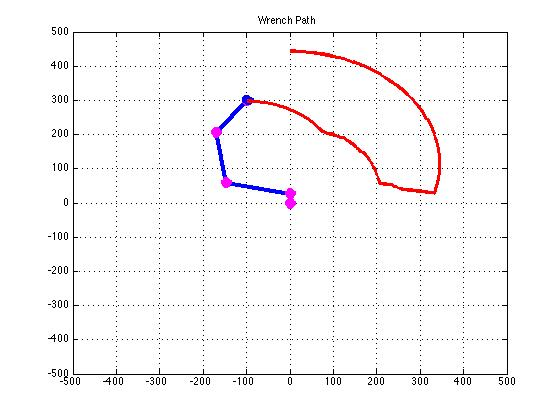
\includegraphics[scale=.3]{PathPics/Wrench_Path.jpg}
\caption{Path When Only Considering The Next State}
\end{subfigure}%
~ 
\begin{subfigure}[b]{0.5\textwidth}
\centering
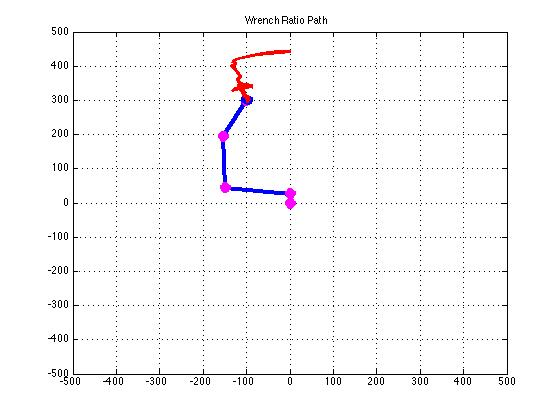
\includegraphics[scale=.3]{PathPics/Wrench_Ratio_Path.jpg}
\caption{Path for Ratio of Torques}
\end{subfigure}

\caption{Paths When Considering Energy To Hold Up an Object}
\label{fig:EnergyPaths2}
\end{figure}\\

\subsection{Kinetic Energy}
The final set of metrics we considered take into account the kinetic energy needed to move from state to state. To simplify this problem we assume the arm is massless except for a mass in the end effector. \\
Once again the Jacobian $J$, comes in handy as a map from from angular velocity to linear velocity. Let $\dot{\theta}$ be the difference in angles between the states $(u,v)$ divided by a time-step $h$. Then the linear kinetic energy of the object the arm is carrying is:
 \[E_{linear} = \frac{1}{2}m \|J_u\dot{\theta}\|^2\]. \\
For angular kinetic energy we approximated the actual value. We assumed that each angle contributes equally to angular kinetic energy and rotates about the same point. This is a significant simplification, but it saves on computation time and complexity. In order to calculate the actual rotation energy, we would need to compute the locations of each joint, not just the end effector in the search, which is at least three times slower. With this approximation our angular kinetic energy is: 
\[E_{angular} = \frac{1}{2}m \left\|\frac{\Delta\theta_1+\Delta\theta_2+\Delta\theta_3)}{h}\right\|^2\]
The final metric we considered was the total kinetic energy between points, which is the sum of the previous two metrics.\\
Figure \ref{fig:KineticPaths} shows the paths for these three metrics. In this path you can see that the total kinetic energy path is identical to the linear kinetic energy path. This is most likely due to the level of approximation in our angular kinetic energy calculations.\\
\begin{figure}[htb]
\centering
\begin{subfigure}[b]{0.33\textwidth}
\centering
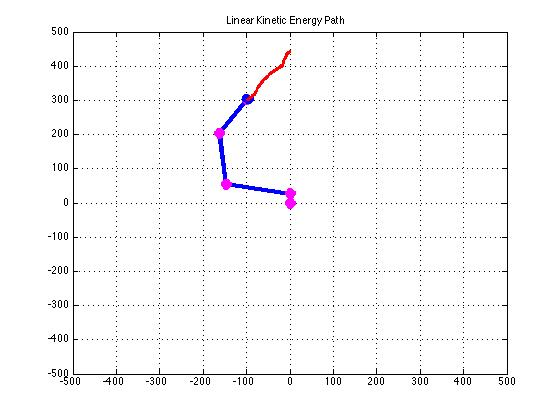
\includegraphics[scale=.33]{PathPics/Energy_Linear_Path.jpg}
\caption{Linear Kinetic Engery Path}
\end{subfigure}%
~ 
\begin{subfigure}[b]{0.33\textwidth}
\centering
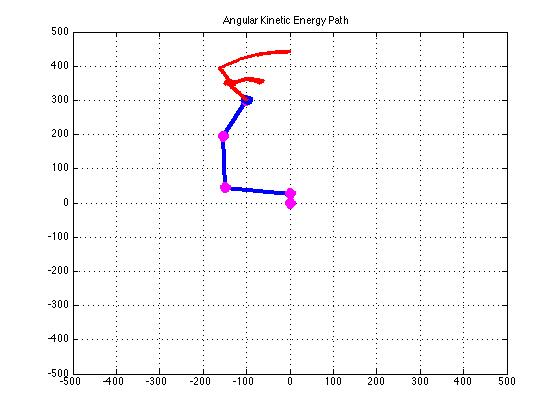
\includegraphics[scale=.33]{PathPics/Energy_Angular_Path.jpg}
\caption{Angular Kinetic Energy Path}
\end{subfigure}%
~ 
\begin{subfigure}[b]{0.33\textwidth}
\centering
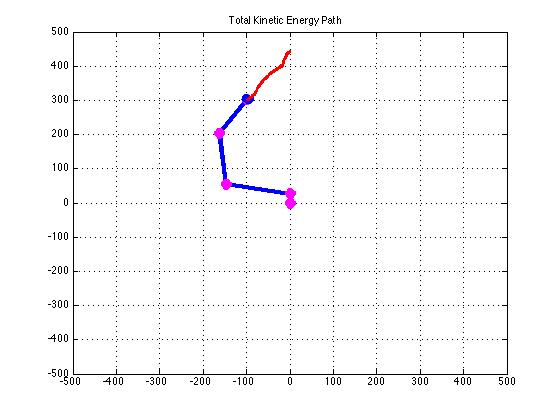
\includegraphics[scale=.33]{PathPics/Energy_Kinetic_Path.jpg}
\caption{Total Kinetic Energy Path}
\end{subfigure}

\caption{Paths When Considering Kinetic Energy}
\label{fig:EnergyPaths2}
\end{figure}\\
\section{Conclusion}
Overall the smoothest path we found was paths that accounted for the total/linear kinetic energy. In this case we specified position and orientation and still found a smooth path to the goal. Using just Euclidean distance if we don't care about orientation the algorithm finds a smooth path. But when trying to find a path with orientation as well it moves into position and then struggles to change orientation without moving too far away from the target. By considering the energies the algorithm can find paths that change orientation on the way even if takes more distance. \\
In practice specifying orientation of the arm will be important. In order to pick up objects, the arm must grip them in a specific way and then place them the right way up. If the path planning can't specify an angle it won't be able to do this. Therefore either including kinetic energy or the cost of holding a position is important for getting smooth paths. Which of these two methods to use depends on the weight of the object you are holding and how long it will stay at each state.
\section{Future Work}
In the future there are several other metrics to consider. One thing to do is to remove the approximations on angular kinetic energy to get a better optimization. Another metric to consider would be the combination of the Kinetic Energy with the cost to hold up an object. These two costs would need to be scaled appropriately to determine which was more important. In general we can continue to work on developing a more accurate physics model of the arm to accurately determine the cost of individual motions. \\
Another way to improve the smoothness of the paths found is to make the tick size smaller. This increases the size of the grid, but lets the robot check more paths. Unfortunately the complexity of the problem is cubic in the grid size, so even small increases in size quickly become too expensive to compute. This is especially true, if the cost of each edge is doing a lot of complicated forward kinematics for each joint and energy calculations.\\
Outside of our simulation, the robot will need to navigate in a house to perform tasks. So it will need to plan a path to move before, it plans a path for the arm. Choosing where to move is another optimization problem in and of itself. There is a shell in the workspace of the arm, where it is more maneuverable and can reach more orientations. Ideally a complete path planning algorithm would move the robot so that the target is in that zone. Alternatively we can relax the constraints on arm position and use the addition of the mobile base to enhance possible manipulations\\
Finally this algorithm needs to move beyond simulation and on to an actual robot. In practice it might be apparent that certain paths are less prone to drifting and accumulating error. This would provided a decisive case for one metric over the other. 
\end{document}